\documentclass{../industrial-development}
\graphicspath{{4-developer`s-activity/}}

\title{Деятельность разработчика в компаниях ИТ-индустрии}
\author{Хорев Никита Олегович, ПИ-21 МО}
\date{}

\begin{document}

\begin{frame}
  \titlepage
\end{frame}


\section{Узкое и широкое понятие разработчика}
\subsection{Узкое понятие деятельности разработчика}
\begin{frame} \frametitle{<<Code monkey>>}
Специально обученный человек, превращающий спецификации в программный код
\end{frame}
\lecturenotes
%что-то написать

\subsection{Широкое понятие деятельности разработчика}
\begin{frame} \frametitle{Задачи разработчика}
  \begin{itemize}
  \item Контроль выполнения планов
	\item Взаимодействие с командой и руководством
	\item Тестирование и разработка тестов
	\item Разработка архитектуры программы
  \end{itemize}
\end{frame}
\lecturenotes
%что-то написать

\section{Контроль выполнения планов и взаимодействие с начальством}
\subsection{Умение сказать <<Да>> и <<Нет>>}
\begin{frame} \frametitle{Почему <<нет>>?}
  \begin{itemize}
  \item Разработчик знает свои возможности
	\item Не надо давать невыполнимые обещания
  \end{itemize}
\end{frame}
\lecturenotes
Разработчик должен здраво оценивать свои возможности и если он не способен выполнить поставленную задачу за указанный срок, ему не стоит просто говорить <<Да>> и затем подставлять себя, работая сверхурочно и в результате всё равно не успев.

\begin{frame} \frametitle{Когда говорить <<нет>>?}
  \begin{itemize}
  \item Чем выше ценность задачи, тем важнее правильно оценить возможности
	\item Признание проблемы нанесёт меньше вреда, чем её сокрытие
  \end{itemize}
\end{frame}
\lecturenotes
Чем выше задача ценнее, там важнее вовремя понять, что она невыполнима и сообщить об этом руководству.
Так будет нанесён меньший ущерб как компании так и репутации, чем если проблема будет замалчиваться до последнего, а к дедлайну окажется, что задача ещё не выполнена.

\begin{frame} \frametitle{Не нужно пытаться}
\begin{flushright}
<<Делай или не делай, не надо пытаться.>>\\
Йода
\end{flushright}
  \begin{itemize}
  \item Слово <<попытаюсь>> --- способ избежать конфликта, а не обещание
  \end{itemize}
\end{frame}
\lecturenotes
Если задача не может быть выполнена, не надо говорить или думать <<я попытаюсь>>.
Это означает, что разработчик до этого момент работал не в полную силу или действовал не оптимально.
Если же он не собирается поменять план или начать действовать по-другому, то обещание <<попытаться>> - просто попытка избежать конфликта.

\begin{frame} \frametitle{Из чего состоит обещание}
\begin{enumerate}
	\item Вы \textit{говорите}, что вы это сделаете
	\item Вы \textit{ответственно относитесь} к своим словам
	\item Вы \textit{выполняете} обещанное
\end{enumerate}
\end{frame}
\lecturenotes
Сказать. Ответственно отнестись. Сделать.\\
Вы говорите, что вы это сделаете.\\
Вы ответственно относитесь к своим словам.\\
Вы выполняете обещанное.\\
Но часто ли нам встречаются люди, которые
выполняют все три части?\\
\begin{itemize}
\itemВы спрашиваете парня из технического отдела, почему сеть работает так медленно, он говорит: «Да, надо бы закупить новые маршрутизаторы». Понятно, что сделано ничего не будет.
\itemВы просите участника группы провести ручное тестирование перед сдачей исходного кода, он отвечает: «Конечно. Постараюсь сделать к концу дня». И почему-то вам кажется, что завтра нужно будет спросить, провел он тестирование или нет.
\itemНачальник входит в комнату и бормочет: «Нам надо работать побыстрее». Вы понимаете, что на самом деле это ВАМ нужно работать побыстрее. Он ничего делать не собирается.
\end{itemize}
Лишь очень немногие люди, обещая что-то, ответственно относятся к своим словам и делают то, что обещали. Некоторые говорят и даже искренне собираются выполнить обещание, но ничего не делают. Гораздо больше людей, которые обещают, совершенно не  обираясь что-то делать. Слышали, как ваши знакомые говорят: «Надо бы заняться спортом, сбросить пяток килограммов», хотя вы прекрасно знаете, что ничего делать они не будут? Такое происходит постоянно.\\
Откуда берется это странное ощущение, что люди в большинстве случаев слишком легкомысленно относятся к своим обещаниям?\\
Что еще хуже, нас порой подводит интуиция. Иногда нам хочется верить, что собеседник ответственно относится к своим словам, хотя в действительности это не так. Мы хотим верить тому, что говорит загнанный в угол разработчик — например, что двухнедельный проект будет завершен за одну неделю… хотя на самом деле это не так.\\
Вместо того чтобы доверять интуиции, можно по некоторым языковым признакам определить, насколько ответственно люди относятся
к своим словам. Правильно выбирая слова, можно решить проблемы с частями 1 и 2 со своей стороны.

\begin{frame} \frametitle{Признаки пустых обещаний}
\begin{itemize}
	\item Нужно/должен
	\item Надеюсь/хорошо бы
	\item Давайте
\end{itemize}
\end{frame}
\lecturenotes
Тщательно выбирайте формулировки, которые вы используете в своих обещаниях, потому что по словам часто можно судить о дальнейшем ходе событий. Если вам не удается подобрать нужные слова, скорее всего, вы недостаточно ответственно относитесь к сказанному или не верите в его выполнимость. Несколько примеров слов и выражений, которые являются характерными признаками пустых обещаний.\\
«Нужно/должен»: «Нам нужно это сделать поскорее», «Мне бы нужно сбросить лишние килограммы», «Кто-то должен об этом позаботиться».\\
«Надеюсь/хорошо бы»: «Надеюсь, это будет сделано к завтрашнему дню», «Надеюсь, мы еще встретимся и поговорим на эту тему», «Хорошо бы выкроить время для этого», «Хорошо бы, чтобы компьютер работал побыстрее».\\
«Давайте»: «Давайте потом встретимся», «Давайте доделаем эту штуку».\\
Если вы начнете обращать внимание на эти слова, то увидите, как часто они звучат вокруг вас — и даже в том, что вы говорите другим. Вы увидите, как мы стараемся избежать ответственности за сказанное. И это недопустимо, если вы или кто-то другой полагается на эти обещания в своей работе. Впрочем, первый шаг уже сделан — вы начинаете узнавать признаки безответственного отношения к обещаниям в окружающих и в себе.\\
Итак, мы знаем, как выглядят пустые обещания. Как узнать настоящее, серьезное обещание?

\begin{frame} \frametitle{Признаки серьезных обещаний}
\begin{itemize}
	\item Вы утверждаете факт того, что ВЫ что-то сделаете, с указанием четкого момента завершения.
	\item Вы принимаете на себя полную ответственность за что-либо перед аудиторией, состоящей минимум из одного человека.
\end{itemize}
\end{frame}
\lecturenotes
У всех выражений из предыдущего раздела есть нечто общее: они предполагают, что «вы» никак не влияете на происходящее и не несете за него ответственности. Во всех случаях люди ведут себя так, словно они являются жертвами ситуации, а не контролируют ее.\\
Но на самом деле лично вы ВСЕГДА можете хоть как-то повлиять на ситуацию, поэтому вы всегда можете ответственно пообещать что-то сделать.\\
Верными признаками серьезных обещаний являются выражения вида «Я сделаю то-то… к такому-то времени…» (например, «Я закончу работу над этим модулем ко вторнику»).\\
Чем так важна эта фраза? Вы утверждаете факт того, что ВЫ чтото сделаете, с указанием четкого момента завершения . Вы говорите не о ком-то другом, а только о себе. Вы говорите о том, что сделаете лично вы. Вы не « надеетесь», что это будет сделано, и не уточняете «если будет время»; вы просто выполните обещанное.\\
Давая такое устное обязательство, вы не сможете отказаться от него без нарушения обещания. Вы сказали, что сделаете, и теперь возможен только один из двух вариантов: вы либо делаете, либо не делаете. Если не делаете, то окружающие могут справедливо спросить, чего же стоят ваши обещания. Вам будет стыдно сказать другим, что вы не сделали обещанное (если они слышали ваше обещание). Неприятная перспектива, не так ли?\\
Вы принимаете на себя полную ответственность за что-либо перед аудиторией, состоящей минимум из одного человека. Вы стоите не
перед зеркалом и не перед экраном компьютера. Вы разговариваете с другим человеком и обещаете что-то сделать. С этого  начинается ответственное обещание. Поставьте себя в ситуацию, которая заставит вас что-то сделать.\\
Переход на язык обязательств поможет вам пройти следующие две фазы: ответственного отношения к словам и выполнения обещанного. Есть несколько причин, из-за которых говорящий может не относиться ответственно к своим обещаниям (или препятствующих их выполнению).

\begin{frame} \frametitle{Выполнение обещания зависит от другого человека }
Сделайте всё возможное с вашей стороны:
\begin{itemize}
	\item Определите зависимости
	\item Создайте интерфейс, абстрагирующий зависимости от инфраструктуры другой группы
	\item Создайте собственную процедуру сборки, в ходе которой выполняются интеграционные тесты
\end{itemize}
\end{frame}
\lecturenotes
Обещайте только то, что находится под вашим полным контролем. Например, если вашей целью является завершение модуля, в работе
над которым также участвует другая группа, вы не можете обещать завершить модуль с полной интеграцией. Однако вы можете обещать выполнить конкретные действия, которые приблизят поставленную цель. Вы можете:\\
1 пообщаться часок-другой с Гарри из инфраструктурной группы, чтобы понять зависимости;\\
2 создать интерфейс, абстрагирующий зависимости модуля от инфраструктуры другой группы;\\
3 встречаться не менее трех раз в неделю с ответственным за сборку, чтобы обеспечить работоспособность ваших изменений в системе сборки, используемой в компании;\\
4 создать собственную процедуру сборки, в ходе которой выполняются интеграционные тесты.\\
Видите разницу?\\
Если конечная цель зависит от кого-то другого, обещайте только конкретные действия, которые способствуют достижению конечной цели.

\begin{frame} \frametitle{Вы не уверены в том, что обещание можно выполнить}
Сделайте всё возможное с вашей стороны:
\begin{itemize}
	\item Убедитесь в достижимости цели
	\item Выполните действия, приближающие достижение цели
\end{itemize}
\end{frame}
\lecturenotes
Даже если конечная цель невозможна, вы можете взять на себя обязательства по выполнению действий, приближающих ее достижение.\\
Более того, проверка достижимости цели может быть одним из таких действий!\\
Вместо того чтобы обещать исправить все 25 оставшихся ошибок до выхода финальной версии (что может быть невозможно), вы обещаете выполнить конкретные действия, приближающие вас к этой цели.\\
Перебрать все 25 ошибок и попытаться воспроизвести их.\\
Пообщаться с автором каждого сообщения об ошибке и увидеть ее воспроизведение.\\
Потратить все оставшееся время на исправление ошибок.

\subsection{Способы оценки времени}
\begin{frame} \frametitle{Что такое оценка?}
\begin{itemize}
  \item Оценка, в первую очередь, это предположение
	\item Она не подразумевает никаких обязательств, вы ничего не обещаете
\end{itemize}
\end{frame}
\lecturenotes
Оценка, прежде всего, является предположением. Она не подразумевает никаких обязательств. Вы ничего не обещаете. Нарушение оценки ни в коей мере не повредит вашей репутации. Мы выдаем оценки, прежде всего, потому, что мы не знаем, сколько времени займет работа.\\
К сожалению, многие разработчики очень слабы в оценках. Дело не в том, что оценка требует какого-то тайного мастерства — вовсе нет. Дело в том, что мы часто не понимаем истинной природы оценки. Оценка — это не число, а распределение. 

\begin{frame} \frametitle{Распределение}
{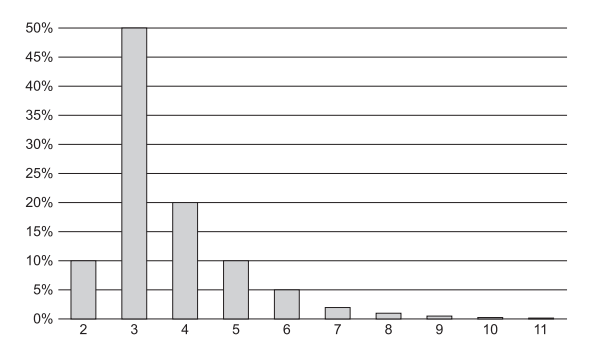
\includegraphics[width=1\linewidth]{time-estimate.png}}
\end{frame}
\lecturenotes
Профессионалы проводят четкое различие между оценками и обязательствами. Они не берут на себя обязательств, пока не будут твердо уверены в успехе. Также они следят за тем, чтобы избегать неявных обязательств. Они по возможности четко оговаривают вероятностное распределение своих оценок, чтобы руководители могли строить соответствующие планы.

\begin{frame} \frametitle{Program Evaluation and Review Technique}
\begin{itemize}
  \item O: оптимистическая оценка
	\item N: номинальная оценка
	\item P: пессимистическая оценка
\end{itemize}
\end{frame}
\lecturenotes
Программа PERT (Program Evaluation and Review Technique) была создана в 1957 году ВМС США для проектирования подводных лодок Polaris. Одним из элементов PERT является способ вычисления оценок.\\
Схема PERT предоставляет очень простой, но исключительно эффективный способ преобразования оценок в вероятностные распределения, подходящие для начальства. При оценке задачи предоставляются три числа (так называемый анализ по трем переменным):\\
O: оптимистическая оценка. Это значение выбирается предельно оптимистично. Задача может быть выполнена за это время только в том случае, если все без исключения пройдет гладко. Более того, чтобы математическая теория сработала, вероятность такого исхода должна быть менее 1\%.\\
N: номинальная оценка (наиболее вероятная).\\
P: пессимистическая оценка. Эта оценка также должна быть крайне предельно пессимистической. В ней следует учесть все возможные неприятности, кроме ураганов, ядерной войны, блуждающих «черных дыр» и других катастроф. Математическая база также работает
только в том случае, если вероятность этого исхода много меньше 1\%.

\begin{frame} \frametitle{Ожидаемая продолжительность задачи}
	\[\mu = \frac{(O + 4N + P)}6\]
	\[\sigma = \frac{(P-O)}6\]
\end{frame}
\lecturenotes
По этим трем оценкам вероятностное распределение описывается следующей формулой: где µ — ожидаемая продолжительность задачи. Для большинства задач оценка получается слегка завышенной, потому что правая часть распределения длиннее левой.
σ — среднеквадратическое отклонение распределения времени выполнения задачи. Фактически это мера неопределенности задачи: если
это число велико, то и неопределенность тоже велика. 

\begin{frame} \frametitle{Оценка времени в группе}
Основной принцип - поиск консенсуса
\begin{itemize}
  \item Широкополосный дельфийский метод: группа обсуждает и оценивает сложность пока не достигнет согласия
	\item Метод быстрого голосования (Покер планирования): сначала происходит обсуждение, а затем участники одновременно показывают ожидаемое время
	\item Аффинная оценка: распределение задач по продолжительности
\end{itemize}
\end{frame}
\lecturenotes
Широкополосный дельфийский метод\\
В 1970-е годы Барри Бем представил метод экспертной оценки, названный «широкополосным дельфийским методом» 1. За прошедшие годы появилось много разновидностей этого метода — как формальных, так и неформальных. Но у всех них есть нечто общее: принцип консенсуса.\\
Стратегия проста. Группа экспертов собирается, обсуждает задачу и оценивает ее сложность. Обсуждение и оценка повторяются до тех пор, пока не будет достигнуто согласие.\\
Покер планирования\\
Всем участникам экспертной группы раздаются карты с разными числами. Участники группы берут карту, которая соответствует их внутренней оценке, и держат ее «рубашкой» вверх, чтобы остальные не видели номинал карты. Затем модератор дает сигнал показать карты.\\
Если оценки согласуются, участники переходят к следующей задаче. В противном случае они продолжают обсуждение, чтобы определить причины расхождений. Цикл повторяется до тех пор, пока их оценки не будут согласованы.\\
Аффинная оценка\\
Все задачи записываются на картах без каких-либо оценок. Экспертная группа стоит возле стола или стены, на которой карты распределены случайным образом. Участники группы не говорят между собой — они просто сортируют карты. Карты задач, которые занимают больше времени, перемещаются направо, а карты меньших задач — налево.\\
Любой участник группы может в любой момент переместить любую карту, даже если она была перемещена другим участником. Карты, перемещенные более h раз, откладываются в сторону для обсуждения.\\
Со временем безмолвная сортировка завершается и начинается обсуждение. Участники разбираются во всех разногласиях по поводу порядка карт. Возможно, для достижения согласия придется провести краткое обсуждение или нарисовать от руки несколько условных схем.

\begin{frame} \frametitle{Закон больших чисел}
\begin{itemize}
  \item При разбиении большой задачи на несколько меньших и независимой их оценке сумма оценок меньших задач будет более точной, чем одна оценка большей задачи. 
\end{itemize}
\end{frame}
\lecturenotes
В оценке заложена ошибка. Собственно, поэтому они и называются оценками. Один из способов контроля ошибок основан на законе больших чисел1. В частности, из этого закона следует, что при разбиении большой задачи на несколько меньших и независимой их оценке сумма оценок меньших задач будет более точной, чем одна оценка большей задачи. Возрастание точности объясняется тем, что погрешности оценки меньших задач взаимно компенсируются.\\
Честно говоря, это утверждение оптимистическое. Погрешности в оценке обычно связаны с недооценкой, а не с переоценкой, так что компенсация вряд ли идеальна. Тем не менее разбиение больших задач с независимой оценкой меньших все равно полезно. Некоторые ошибки взаимно компенсируются, а разбиение задачи поможет лучше понять ее суть и выявить возможные неожиданности.

\subsection{Под давлением}
\begin{frame} \frametitle{Как избежать давления}
\begin{itemize}
  \item Избегать невыполнимых обязательств
  \item Сохранять чистоту
	\item Придерживаться оптимальных методов
\end{itemize}
\end{frame}
\lecturenotes
Обязательства\\
Важно избегать принятия обязательств на сроки, в соблюдении которых вы не уверены. Бизнес всегда будет стараться добиться от вас таких обязательств, потому что он хочет полностью исключить риск. А мы должны позаботиться о том, чтобы риски объективно оценивались и  представлялись бизнесу таким образом, чтобы тот мог правильно управлять ими. Принятие нереалистичных обязательств противоречит этой цели и оказывает плохую услугу как бизнесу, так и нам самим.\\
Иногда обязательства принимаются за нас. Иногда мы вдруг узнаем, что начальство что-то пообещало заказчику, не проконсультировавшись с нами. В таких случаях профессиональная честь требует помочь бизнесу найти возможность выполнения этих обязательств. Тем не менее та же профессиональная честь не требует от нас принятия этих обязательств.\\
Различие достаточно принципиальное. Профессионал всегда помогает бизнесу найти способ достижения его целей, но он не всегда принимает на себя обязательства, принятые за него. В конечном итоге, если нам не удастся выполнить обязательства, принятые за нас, то ответственность за это должен нести тот, кто эти обязательства принял.\\
Легко сказать… Когда ваш бизнес разваливается, а зарплата откладывается из-за нарушенных обязательств, трудно устоять перед давлением. Но если вы вели себя профессионально, то по крайней мере сможете искать новую работу с достоинством и чистой совестью.\\
Как сохранить чистоту\\
Чтобы двигаться быстро и не нарушать сроков, в коде необходимо сохранять чистоту. Профессионал не поддается искушению устроить грязь в коде, чтобы быстро двигаться вперед. Грязно — всегда значит медленно!\\
Сохранение чистоты в системе, коде и архитектуре помогает избежать давления. Это вовсе не означает, что вы должны до бесконечности
«полировать» код. Речь о другом: о непримиримом отношении к грязи. Мы знаем, что грязь замедлит нашу работу, приведет к срыву сроков
и нарушению обязательств. Соответственно мы всеми силами пытаемся сохранить результаты нашей работы в настолько чистом состоянии, насколько это возможно.\\
Дисциплина в кризисных ситуациях\\
Чтобы понять, во что вы по-настоящему верите, понаблюдайте за собой в кризисной ситуации. Если во время кризиса вы не отклоняетесь от своих рабочих методов, значит вы действительно убеждены в их эффективности. Если вы следуете методологии разработки через тестирование (TDD) в обычное время, но отказываетесь от нее во время кризиса, значит вы не верите в полезность TDD. Если ваш код остается чистым в обычное время, а в кризис вы разводите в нем грязь, значит вы не верите, что грязь замедляет вашу работу. Если вы используете парное программирование во время кризиса, но не в обычной ситуации, значит вы полагаете, что парное программирование эффективнее индивидуального. Выберите те методы, с которыми вы комфортно ощущаете себя в кризисной ситуации. А потом используйте их постоянно. Использование этих методов — лучший способ избежать кризиса.\\
Не изменяйте свое поведение в напряженной ситуации. Если ваши методы действительно оптимальны, то они должны соблюдаться даже в самые тяжелые времена

\begin{frame} \frametitle{Как вести себя в тяжелой ситуации}
\begin{itemize}
  \item Без паники
  \item Взаимодействуйте
\end{itemize}
\end{frame}
\lecturenotes
Предотвращение и устранение кризисов — дело, конечно, хорошее, но иногда вы оказываетесь под давлением независимо от своего желания. Иногда проект просто занимает больше времени, чем планировалось изначально. Иногда исходная архитектура оказывается неверной и ее приходится перерабатывать. Иногда вы лишаетесь ценного работника или заказчика. Иногда вы принимаете обязательство, которое не удается выполнить. Что желать в таких случаях?\\
Без паники\\
Возьмите свой стресс под контроль. Бессонные ночи не помогут выполнить работу быстрее. Ругань тоже не поможет. Но самое худшее, что вы можете сделать, — это спешка! Боритесь с этим искушением любой ценой. Спешка только затянет вас еще глубже на дно.\\
Наоборот, притормозите и продумайте задачу. Проложите курс к лучшему из возможных решений, а затем двигайтесь по этому курсу в разумном, стабильном темпе.\\
Взаимодействие\\
Уведомите свою группу и начальство о неприятностях. Изложите свой план по выходу из кризиса. Обратитесь к ним за информацией и советом. Избегайте сюрпризов. Ничто не сердит людей и не делает их менее рациональными так, как сюрпризы. Сюрпризы повышают уровень стресса десятикратно.

\subsection{Взаимодействие с начальством}
\begin{frame} \frametitle{Понимание целей проекта}
\begin{itemize}
  \item Забота об интересах работодателя
  \item Понимание цели проекта
\end{itemize}
\end{frame}
\lecturenotes
Первая обязанность профессионального программиста — заботиться об интересах своих работодателей. Это означает, что вы должны общаться со своими начальниками, бизнес-аналитиками, тестерами и другими участниками группы, чтобы глубоко понимать коммерческие цели проекта. Никто не заставляет вас становиться экспертом в области бизнеса.\\
Просто нужно понимать, зачем вы пишете свой код и какую пользу он приносит вашей фирме.\\
Худшее, что может сделать профессиональный программист, — в блаженном неведении укрыться в технологическом убежище, когда бизнес горит и рушится вокруг него. Ваша работа — удерживать бизнес на плаву!\\
Итак, профессиональный программист должен выделить время на изучение коммерческой стороны дела. Он говорит с пользователями о программном продукте, с которым они работают. Он общается с людьми из отдела продаж и маркетинга по поводу возникающих проблем. Он говорит с начальством, чтобы понять как краткосрочные, так и долгосрочные цели группы.\\
Короче говоря, профессиональный программист обращает внимание на корабль, на котором он плывет.

\section{Взаимодействие с другими разработчиками}
\subsection{Взаимопомощь}
\begin{frame} \frametitle{Как помогать другим}
\begin{itemize}
  \item Быть готовым
  \item Выделить на помощь время
\end{itemize}
\end{frame}
\lecturenotes
Ответственные программисты должны быть готовы помогать друг другу. Программист, который изолируется в своем офисе или кабинке и отказывается отвечать на вопросы других, нарушает профессиональную этику. Ваша работа не настолько важна, чтобы вы не могли выделить немного времени на помощь другим.\\
Честь профессионала обязывает предложить ближним помощь тогда, когда это потребуется. Это не означает, что вы должны отказаться от «личного времени». Конечно, оно необходимо, но к его выбору следует подойти вежливо и честно. Например, вы можете сообщить, что между 10:00 и полуднем вас нельзя беспокоить, а с 13:00 до 15:00 ваша дверь открыта для других.\\
Также будьте внимательны к состоянию работы ваших коллег. Если кто-то испытывает затруднения, предложите помощь. Просто удивительно, насколько эффективной порой оказывается такая помощь. Дело не в том, что вы намного умнее своего коллеги; просто свежая точка зрения нередко становится мощным катализатором для решения проблем.\\
Когда вы кому-то помогаете, сядьте и напишите код вместе. Запланируйте на помощь не менее часа. Возможно, вам понадобится меньше времени, но торопиться не стоит. Сосредоточьтесь на задаче и приложите максимум усилий. Скорее всего, вы в конечном итоге от такого сотрудничества получите больше, чем отдадите.

\begin{frame} \frametitle{Как принимать помощь}
\begin{itemize}
  \item Научиться просить о помощи
\end{itemize}
\end{frame}
\lecturenotes
Когда кто-то предлагает вам помощь, будьте признательны. Примите помощь с благодарностью и отнеситесь к ней со всем вниманием. Не отказывайтесь от помощи, потому что вам не хватает времени. Выделите на разговор около минут 30. Если особой пользы от предложенной помощи не видно, вежливо извинитесь и завершите беседу с благодарностью. Помните: профессионализм обязывает вас не только предлагать, но и принимать предложенную помощь.\\
Научитесь просить о помощи. Когда вы зашли в тупик или не можете разобраться в задаче, попросите других помочь вам. Если вы находитесь в общей комнате, просто скажите: «Мне нужна помощь». В остальных случаях можно воспользоваться Твиттером, электронной почтой или телефоном. Обратитесь за помощью — в конце концов, это также является делом профессиональной этики. Непрофессионально оставаться в тупике, когда помощь так доступна.\\
Думаете, я сейчас нарисую радужную картину — хор поет проникновенную песню, пушистые зайчики прыгают на спины единорогам и все дружно отправляются к радуге надежды и изменений? Нет, не совсем так. Видите ли, программисты обычно бывают самонадеянными, эгоцентричными интровертами. Мы идем в эту область не потому, что мы любим людей. Большинство из нас приходит в программирование, потому что нам нравится концентрироваться на мелочах, жонглировать множеством абстрактных концепций и иным образом доказывать себе, что мы являемся обладателями выдающегося интеллекта, — а вовсе не для того, чтобы разбираться с досадными сложностями других людей.\\
Да, это стереотип. Да, это обобщение со множеством исключений. Однако реальность такова, что программисты не склонны к сотрудничеству. Тем не менее сотрудничество играет исключительно важную
роль в эффективном программировании. А раз для многих из нас оно не является инстинктом, значит, нам нужны методологии, которые заставляют нас сотрудничать.

\subsection{Встречи}
\begin{frame} \frametitle{Встречи}
Две истины о встречах:
\begin{itemize}
  \item Встречи необходимы
  \item Встречи часто оказываются бесплодной тратой времени
\end{itemize}
\end{frame}
\lecturenotes
Когда вы в следующий раз будете проводить рабочую встречу, посчитайте затраты на нее. Результат вас сильно удивит.
Две истины о встречах:
1) встречи необходимы;
2) встречи часто оказываются бесплодной тратой времени.
Часто эти две истины относятся к одной и той же встрече. Одним участникам встреча кажется бесценной, другим — лишней или бесполезной. Профессионалы знают, что встречи обходятся дорого. Они также знают, что их собственное время драгоценно; им нужно писать код и выдерживать график. По этой причине они активно сопротивляются посещению встреч, которые не приносят немедленной и значительной пользы.

\begin{frame} \frametitle{Отказ от участия}
\begin{itemize}
  \item Не обязательно посещать \textbf{все} встречи.
  \item Человек, приглашающий вас на встречу, не отвечает за управление вашим временем — за него отвечаете только вы
\end{itemize}
\end{frame}
\lecturenotes
Вы не обязаны посещать каждую встречу, на которую вас приглашают. Более того, посещать слишком много встреч непрофессионально. Время нужно расходовать разумно. Будьте очень осмотрительны с выбором встреч, которые нужно посетить или от которых нужно вежливо отказаться. Человек, приглашающий вас на встречу, не отвечает за управление вашим временем — за него отвечаете только вы. Таким образом, получив приглашение, не принимайте его, если только ваше участие не объясняется немедленной и значительной необходимостью для текущей работы.\\
Иногда встреча посвящена теме, которая представляет для вас интерес, но не является строго необходимой. Решайте сами, сможете ли вы выделить для нее время. Будьте осторожны — такие встречи способны поглотить все ваше рабочее время.\\
Иногда вы знаете, что ваше участие может принести пользу, но встреча не является непосредственно значимой для того, чем вы сейчас занимаетесь. Решайте, компенсируются ли потери для вашего проекта пользой для других проектов. Возможно, это прозвучит цинично, но вы в первую очередь отвечаете за свои проекты. Тем не менее взаимопомощь групп часто приносит пользу, так что вы можете обсудить возможность своего участия со своей группой и начальством.\\
Иногда с просьбой о вашем присутствии на встрече к вам обращается какое-нибудь авторитетное лицо — например, технический специалист очень высокого уровня или руководитель другого проекта. Вам придется решать, перевешивает ли этот авторитет ваш рабочий график. Как и в предыдущем случае, в принятии решения может помочь группа или начальство.\\
Одна из самых важных обязанностей вашего руководителя — удерживать вас от участия в лишних встречах. Хороший руководитель более чем охотно защитит ваш отказ от участия, потому что ваше время представляет для него такую же ценность, как и для вас

\begin{frame} \frametitle{Споры и разногласия}
\begin{itemize}
  \item Любой спор, который не удается завершить за 5 минут, не может быть решен обсуждением
  \item Избегайте встреч, на которых присутствует только одна из спорящих сторон
\end{itemize}
\end{frame}
\lecturenotes
Кент Бек однажды сказал очень важную вещь: «Любой спор, который не удается завершить за 5 минут, не может быть решен обсуждением». Если спор занимает слишком много времени, значит, не существует четких доказательств в пользу одной из сторон. В таких ситуациях спор обычно имеет религиозную подоплеку, а не базируется на фактах.\\
Технические разногласия порой заходят за край. У каждой стороны имеются всевозможные обоснования своей позиции, которые редко подкрепляются данными. Без данных любой спор, который не приходит к согласию за несколько минут (от 5 до 30), попросту не способен прийти к согласию. Единственное, что можно сделать в такой ситуации, — это раздобыть данные.\\
Некоторые люди пытаются выиграть в споре за счет демонстрации характера. Они кричат, пытаются давить или изображают снисходительность. Это не важно; сила воли не может разрешить спор на продолжительное время. Данные — могут.\\
Другие занимают пассивно-агрессивную позицию. Они соглашаются просто для того, чтобы закончить спор, а затем саботируют результат, отказываясь участвовать в решении. Они говорят себе: «Вы так хотели, вот теперь сами и разбирайтесь». Вероятно, это худший из вариантов непрофессионального поведения. Никогда, никогда не поступайте подобным образом. Если вы соглашаетесь, то вы обязаны участвовать.\\
Как получить данные, необходимые для урегулирования разногласий? Иногда можно провести эксперимент, устроить имитацию или моделирование. А иногда лучше всего попросту бросить монетку, чтобы выбрать один из двух путей.\\
Если все получилось, значит, этот путь был работоспособным. Если возникли проблемы — вернитесь и опробуйте другой путь. Заранее согласуйте время и набор критериев, по которым будет приниматься
решение об отказе от выбранного пути.\\
Остерегайтесь встреч, которые проводятся только для подавления разногласий и привлечения поддержки одной из сторон. Также избегайте встреч, на которых присутствует только одна из спорящих сторон.\\
Если спор необходимо урегулировать, попросите каждую сторону изложить свои аргументы группе не более чем за 5 минут, после чего проведите голосование. Вся встреча займет не более 15 минут

\subsection{Работа в группе}
\begin{frame} \frametitle{Формирование группы}
\begin{itemize}
  \item Группы формируются не сразу. Между участниками постепенно налаживаются отношения
  \item В группу должны входить программисты, тестеры, аналитики и руководитель проекта
\end{itemize}
\end{frame}
\lecturenotes
Группы формируются не сразу. Между участниками постепенно налаживаются отношения. Они учатся работать друг с другом, узнают странности, сильные и слабые стороны своих коллег. Со временем
участники «притираются» друг к другу.\\
В «притертой» группе есть что-то волшебное: она способна творить чудеса. Участники понимают друг друга, поддерживают и требуют максимальной отдачи. Благодаря их взаимодействию достигаются результаты.\\
«Притертая» группа обычно содержит около дюжины участников. Их может быть и больше (до 20) или меньше (до 3), но оптимальный размер обычно где-то около 12. В группу должны входить программисты, тестеры и аналитики. И у нее должен быть руководитель проекта.\\
Соотношение численности программистов и тестеров/аналитиков изменяется в широких пределах, но пропорция 2:1 вполне разумна. Таким образом, хорошо «притертая» группа из 12 человек может состоять из семи программистов, двух тестеров, двух аналитиков и руководителя проекта.\\
Аналитики разрабатывают требования и пишут для них автоматизированные приемочные тесты. Тестеры тоже пишут автоматизированные приемочные тесты, но отличаются от аналитиков направленностью. И те и другие пишут тесты, но аналитики ориентируются на коммерческую ценность, а тестеры — на правильность работы кода. Аналитики пишут «оптимистичные» тесты, а тестеры беспокоятся о том, что
может пойти не так, и пишут тесты для выявления сбоев и граничных случаев.\\
Руководитель проекта следит за прогрессом и принимает меры к тому, чтобы группа понимала сроки и приоритеты. Один из участников группы может совмещать выполнение своих обязанностей с ролью наставника, ответственного за соблюдение технологических процессов и методов. Он становится своего рода «коллективной совестью», когда у группы возникает соблазн нарушить правила под давлением сроков.\\
Созревание\\
Чтобы участники разобрались в своих различиях и договорились между собой, а группа действительно «притерлась», потребуется время. Процесс может занять полгода или даже год. Но когда это случается, происходит чудо. «Притертая» группа вместе планирует, вместе решает задачи, вместе разбирается с проблемами и добивается результатов. Разбивать такие группы только из-за завершения проекта слишком расточительно. Лучше сохранить группу в прежнем составе и поручать ей новые проекты.\\
Что сначала — группа или проект?\\
Банки и страховые компании пытались формировать группы на базе проектов. Такой подход неверен в принципе: группы просто не могут «притереться». Участники работают над проектом в течение короткого времени, притом посвящая ему лишь часть своего рабочего времени, а следовательно, не имеют возможности сработаться.\\
Профессиональные фирмы-разработчики поручают проекты существующим «притертым» группам, а не формируют группы для конкретного проекта. «Притертая» команда может вести сразу несколько проектов и распределять работу в соответствии со своими предпочтениями, квалификацией и способностями участников.

\begin{frame} \frametitle{Управление группой}
\begin{itemize}
  \item Группы формируются не сразу. Между участниками постепенно налаживаются отношения
  \item В группу должны входить программисты, тестеры, аналитики и руководитель проекта
\end{itemize}
\end{frame}
\lecturenotes
У каждой группы имеется определенная скорость работы, а проще говоря, объем работы, выполняемый за фиксированный промежуток времени. Некоторые группы измеряют свою скорость в пунктах в неделю
(пункты — единица сложности). Функциональность каждого проекта, над которым работает группа, разбивается на блоки, сложность которых оценивается в пунктах. В дальнейшем производительность группы оценивается по количеству пунктов, реализованных за неделю.\\
Скорость — статистическая метрика. Группа может реализовать 38 пунктов в одну неделю, 42 пункта в другую и 25 в третью. По мере накопления данных вычисляется усредненный показатель. Руководство может задать цели для каждого проекта, Например, если средняя скорость группы равна 50 и группа работает над тремя проектами, руководство может попросить группу распределить усилия
в пропорции 15/15/20.\\
Помимо того что над проектами работает «притертая» команда, у этой схемы есть и другое преимущество. В напряженной ситуации бизнессторона может сказать: <<Проект B в критическом состоянии; в следующие три недели направьте на него 100\% усилий>>\\
Столь быстрое перераспределение приоритетов практически невозможно со случайно подобранными группами, тогда как «притертая» группа, работающая над двумя или тремя проектами одновременно, легко выполняет подобные «развороты на месте».\\
Дилемма владельца проекта\\
Один из аргументов против метода, за который я выступаю, заключается в том, что он частично лишает владельцев проекта уверенности и власти. Владельцы проекта, для которого была создана специальная группа, могут рассчитывать на полную отдачу этой группы. Они знают, что формирование и роспуск группы обходится недешево, поэтому бизнес не будет отнимать у них группу по краткосрочным тактическим соображениям.\\
С другой стороны, если проекты даются «притертым» группам и эти группы ведут сразу несколько проектов, бизнес может менять приоритеты по своему усмотрению. Из-за этого владелец проекта менее уверен в будущем. У него могут внезапно отобрать ресурсы, на которые он рассчитывает

\subsection{Обучение}
\begin{frame} \frametitle{Квалификации}
\begin{itemize}
  \item Мастер
  \item Ремесленник
	\item Ученик
\end{itemize}
\end{frame}
\lecturenotes
Период ученичества\\
Итак, как же молодые выпускники должны вливаться в ряды профессиональных программистов? Какой путь они должны пройти? С какими препятствиями столкнуться? Каких целей они должны достичь? Давайте рассмотрим профессиональные уровни программистов по убыванию квалификации.\\
Мастер\\
К этой категории относятся программисты, возглавлявшие более одного серьезного программного проекта. Как правило, они имеют более чем 10-летний стаж работы с разными системами, языками и операционными системами. Они умеют руководить и координировать работу нескольких команд, являются квалифицированными проектировщиками и разработчиками архитектур и могут запросто запрограммировать что угодно. Им предлагались руководящие должности, но они либо отклонили предложение, либо вернулись обратно после согласия, либо интегрировали их в свою основную техническую роль. Для поддержания своей квалификации в этой роли они читают техническую литературу, учатся, тренируются, работают и учат. Именно мастера несут ответственность за реализацию проекта с технической стороны.\\
Ремесленник\\
Рядовые программисты — обученные, компетентные и энергичные. В этот период своей карьеры они учатся работать в группах и выполнять функции руководителя. Они хорошо разбираются в современной
технологии, но обычно им не хватает опыта работы с разнообразными системами. Обычно ремесленник знает один язык, одну систему, одну платформу; но он старается узнать больше. Стаж работы в этой категории сильно различается; среднее значение составляет около 5 лет. На ближнем конце оси находятся недавние ученики, а на дальнем — зарождающиеся мастера.\\
Наставниками ремесленников являются мастера или более опытные ремесленники. Молодым ремесленникам редко предоставляется самостоятельность. За их работой плотно наблюдают, а их код проверяется. По мере накопления опыта самостоятельность растет, контроль становится менее прямолинейным и в конечном итоге преобразуется в равноправное рецензирование кода.
Ученики/интерны\\
Карьера выпускника начинается с позиции ученика. У учеников нет никакой самостоятельности — их очень плотно контролируют ремесленники. Сначала ученики вообще не выполняют никаких задач, просто помогая ремесленникам. Это должно быть время чрезвычайно интенсивного парного программирования. Именно в это время изучаются и закрепляются методы и приемы. Именно в это время закладывается фундамент системы профессиональных ценностей.\\
Ремесленники становятся учителями. Они следят за тем, чтобы ученики знали принципы и паттерны проектирования, методы и ритуалы. Ремесленники обучают их TDD, рефакторингу, искусству оценки и т. д. Они назначают ученикам книги, раздают упражнения и учебные задачи; они следят за их прогрессом.\\
Ученичество должно длиться не менее года. За это время, если ремесленники пожелают принять новичка в свои ряды, они обращаются к мастерам с рекомендацией. Мастера изучают новичка — как в личном собеседовании, так и посредством анализа достижений. Если мастера соглашаются, то ученик переходит в ремесленники.\\
Реальность\\
И снова скажу, что это описание идеализированное и гипотетическое. Но если немного изменить терминологию, вы поймете, что оно не так уж сильно отличается от сегодняшней ситуации. Выпускников опекают молодые руководители групп, которых опекают руководители проектов и т. д. Проблема в том, что в большинстве случаев опека имеет нетехническую природу! В большинстве компаний технического контроляь нет вообще. Программисты получают прибавки и повышения, потому
что… потому что так положено.\\
Различия между сегодняшним положением дел и моей идеализированной программой заключается в ориентированности последней на техническое обучение, опеку и контроль. Оно проявляется в самом
представлении о том, что профессиональные ценности и техническую сметку нужно объяснять, культивировать и взращивать. В нашем современном стерильном подходе отсутствует ответственность старших за обучение молодежи.


\section{Тестирование}
\subsection{Test driven development}
\begin{frame} \frametitle{Разработка через тестирование}
\begin{itemize}
  \item Новый рабочий код пишется только после того, как будет написан модульный тест, который не проходит.
  \item Вы пишете ровно такой объем кода модульного теста, какой необходим для того, чтобы этот тест не проходил (если код теста не компилируется, считается, что он не проходит).
	\item Вы пишете ровно такой объем рабочего кода, какой необходим для прохождения модульного теста, который в данный момент не проходит.
\end{itemize}
\end{frame}
\lecturenotes
За прошедшие годы о TDD было написано много противоречивых статей и блогов. На первых порах встречалась серьезная критика и сомнения, но в наши дни все дискуссии завершены. Кто бы что ни говорил, TDD работает.\\
Я знаю, что это утверждение кажется слишком жестким и односторонним, но в конце концов, хирургам уже не нужно доказывать полезность мытья рук. И я не думаю, что программистам нужно защищать TDD.\\
Как можно называть себя профессионалом, если вы не знаете, что весь ваш код работает? А как можно знать, что весь ваш код работает, если вы не тестируете его при каждом внесении изменений? А как тестировать код при каждом внесении изменений, не имея автоматизированных модульных тестов с очень высоким покрытием? Но можно ли создать автоматизированные модульные тесты с очень высоким покрытием без применения TDD?\\
Впрочем, последнее предложение стоит рассмотреть более подробно. Что же это, собственно, такое — TDD?\\
Три закона TDD\\
1. Новый рабочий код пишется только после того, как будет написан модульный тест, который не проходит.\\
2. Вы пишете ровно такой объем кода модульного теста, какой необходим для того, чтобы этот тест не проходил (если код теста не компилируется, считается, что он не проходит).\\
3. Вы пишете ровно такой объем рабочего кода, какой необходим для прохождения модульного теста, который в данный момент не проходит.\\
Эти три закона заставляют вас использовать рабочий цикл продолжительностью около 30 секунд. Сначала вы пишете маленькую часть модульного теста. За эти считанные секунды вы упоминаете в коде
имя класса или функции, которые еще не были написаны; естественно, модульный тест не компилируется. Следовательно, далее вы должны написать рабочий код, с которым тест откомпилируется. Но писать больше кода нельзя, поэтому вы переходите к написанию дополнительного кода модульного теста.\\
Цикл прокручивается снова и снова. Добавляем небольшой фрагмент в тестовый код. Добавляем небольшой фрагмент в рабочий код. Два кодовых потока растут одновременно, превращаясь во взаимодополняющие компоненты. Соответствие между тестами и рабочим кодом напоминает соответствие между антителом и антигеном.

\subsection{Приёмочные тесты}
\begin{frame} \frametitle{Приемочные тесты}
  \begin{block}{Определение}
	Тесты, написанные при совместном участии заинтересованных сторон и программистов для проверки выполнения требований.
  \end{block}
\end{frame}
\lecturenotes
Приемочные тесты\\
Термин «приемочные тесты» перегружен множеством значений. Одни полагают, что речь идет о тестах, выполняемых пользователями перед приемкой очередной версии продукта. Другие понимают под этим термином контроль качества. Здесь под термином «приемочные тесты» понимаются тесты, написанные при совместном участии заинтересованных сторон и программистов для проверки выполнения
требований.

\begin{frame} \frametitle{Что такое <<выполнено>>?}
Когда разработчик говорит, что он выполнил свою задачу, что он имеет в виду?
\begin{itemize}
  \item Что он готов передать свой код в эксплуатацию с полной уверенностью?
  \item Что его код готов к прохождению контроля качества?
	\item Что он дописал свой код и даже смог один раз выполнить его, но еще не подвергал тестированию?
\end{itemize}
\end{frame}
\lecturenotes
Что такое «выполнено»?\\
Одна из самых распространенных неоднозначностей, с которыми сталкиваются профессиональные разработчики, связана с самим понятием «выполнения». Когда разработчик говорит, что он выполнил свою задачу, что он имеет в виду? Что он готов передать свой код в эксплуатацию с полной уверенностью? Что его код готов к прохождению контроля качества? А может, что он дописал свой код и даже смог один раз выполнить его, но еще не подвергал тестированию?
Есть группы, имеющие разные представления о терминах «выполнено» и «готово». Где-то могут использоваться термины «сделано» и «совсем сделано». У профессиональных разработчиков есть только одно определение: выполнено — значит выполнено. Сделано — значит, что весь код написан, все тесты пройдены, служба контроля качества и ключевые участники приняли результат. Сделано.\\
Но как добиться такого уровня выполнения, не снижая темпа перехода между итерациями? Нужно создать набор автоматизированных тестов, прохождение которых означает выполнение всех перечисленных условий! Если приемочные тесты вашей подсистемы проходят успешно, значит, работа выполнена.\\
Профессиональные разработчики расширяют определение требований до автоматизированных приемочных тестов. Они общаются с ключевыми участниками и специалистами по контролю качества, стремясь к тому, чтобы автоматизированные тесты полностью отражали определение «выполнения».

\begin{frame} \frametitle{Автотесты}
  \begin{block}{}
Приемочные тесты всегда должны быть автоматизированными
	\end{block}
\end{frame}
\lecturenotes
Приемочные тесты всегда должны быть автоматизированными. В других моментах жизненного цикла программных продуктов находится место для ручного тестирования, но такие тесты никогда не должны выполняться вручную. Причина проста: затраты.\\
ые разработчики не допускают возникновения подобных ситуаций. Затраты на проведение автоматизированных тестов настолько малы по сравнению с затратами на ручное тестирование, что написание сценариев, запускаемых вручную, не имеет никакого
экономического смысла. Профессиональные разработчики считают своей обязанностью проследить за тем, чтобы приемочные тесты проводились в автоматизированном режиме.\\
Существует множество программных инструментов (как коммерческих, так и с открытым кодом), автоматизирующих приемочные тесты. FitNesse, Cucumber, cuke4duke, robot framework и Selenium — этот список далеко не полон. Во всех этих инструментах автоматизированные тесты определяются в такой форме, что даже не-программисты могут
читать их, понимать и даже создавать.

\begin{frame} \frametitle{Обсуждение тестов}
\begin{itemize}
  \item Авторы тестов — люди, и они тоже допускают ошибки
  \item Не надо занимать позицию <<Как написано в тесте, так я и сделаю>>
	\item Профессионал обязан помочь своей группе создать программу
настолько качественную, насколько это возможно
\end{itemize}
\end{frame}
\lecturenotes
Обсуждение тестов и пассивно-агрессивная позиция\\
Авторы тестов — люди, и они тоже допускают ошибки. Иногда при переходе к реализации становится очевидно, что тест выглядит бессмысленно. Тесты бывают слишком запутанными или громоздкими.\\
Они могут базироваться на нелепых предпосылках. А иногда они попросту неверны. Все это может быть весьма неприятно, если вы — разработчик, который должен обеспечить прохождение теста.\\
Ваша задача как профессионального разработчика — обсудить ситуацию с автором теста для его улучшения. Никогда не выбирайте пассивно-агрессивную позицию, когда вы говорите себе: «Как написано в тесте, так я и сделаю».\\
Помните: профессионал обязан помочь своей группе создать программу настолько качественную, насколько это возможно. А это означает, что все должны уделять внимание возможным ошибкам и промахам коллег и совместно работать над их исправлением.

\begin{frame} \frametitle{Модульные тесты как документация архитектуры}
\begin{itemize}
  \item Модульные (unit) тесты пишутся программистами для программистов
  \item Приемочные тесты создаются бизнесменами для бизнесменов
	\item Главная цель модульных тестов — формальное документирование архитектуры, структуры и поведения системы.
\end{itemize}
\end{frame}
\lecturenotes
Не путайте приемочные тесты с модульными (unit tests). Модульные тесты пишутся программистами для программистов. Они представляют собой формальные архитектурные документы с описанием нижнего уровня структуры и поведения кода. Их читателями являются не бизнесмены, а программисты.\\
Приемочные тесты создаются бизнесменами для бизнесменов (даже если в конечном итоге их пишете вы, разработчик). Они представляют собой формальные описания требований, определяющие поведение системы с точки зрения бизнеса. Их читателями являются бизнесмены и программисты.\\
Возможно, у кого-то возникнет соблазн избавиться от лишней работы, предположив, что тесты двух видов избыточны. Но хотя модульные и приемочные тесты часто тестируют одно и то же, никакой избыточности в них нет.\\
Во-первых, даже если они тестируют одно и то же, при этом используются разные пути и механизмы. Модульные тесты углубляются во внутреннюю реализацию системы и вызывают методы конкретных классов. Приемочные тесты обращаются к системе на значительно более высоком уровне — уровне API или даже уровне пользовательского
интерфейса. Таким образом, пути выполнения этих тестов сильно различаются.\\
Но настоящая причина, по которой эти тесты нельзя назвать избыточными, заключается в том, что тестирование не является их главной функцией. Тот факт, что они что-то проверяют, вторичен. Модульные и приемочные тесты прежде всего являются документами и лишь потом — тестами. Их главная цель — формальное документирование архитектуры, структуры и поведения системы. Автоматическая проверка архитектуры, структуры и поведения чрезвычайно полезна, но истинной целью является именно документирование.

\subsection{Стратегия тестирования}
\begin{frame} \frametitle{Контроль качества не должен находить дефекты}
  \begin{block}{}
	Группа разработки должна стремиться к тому, чтобы контроль качества не выявлял никаких дефектов
  \end{block}
\end{frame}
\lecturenotes
Несмотря на то что в вашей компании может существовать отдельная группа контроля качества, занимающаяся тестированием программных продуктов, группа разработки должна стремиться к тому, чтобы контроль качества не выявлял никаких дефектов.\\
Конечно, вряд ли эта цель будет достигаться постоянно. В конце концов, когда группа умных людей решительно и непреклонно стремится выявить все дефекты и недостатки продукта, она наверняка чего-нибудь найдет. И все же каждый раз, когда служба контроля качества что-нибудь обнаруживает, это должно стать тревожным сигналом для
разработчиков. Они должны спросить себя, как это произошло, и принять меры для предотвращения подобных инцидентов в будущем.

\begin{frame} \frametitle{QA – не враг, а часть команды}
  \begin{block}{}
	Служба контроля качества и группа разработки совместно работают для повышения качества системы, а оптимальная роль для специалистов по контролю качества должна заключаться в создании спецификаций и описании характеристик системы.
  \end{block}
\end{frame}
\lecturenotes
Из предыдущего раздела может сложиться впечатление, что служба контроля качества и группа разработки противодействуют друг другу, что их отношения имеют антагонистический характер. Этого быть не должно. Служба контроля качества и группа разработки совместно работают для повышения качества системы, а оптимальная роль для специалистов по контролю качества должна заключаться в создании спецификаций и описании характеристик системы.\\
Создание спецификаций\\
Служба контроля качества должна работать совместно с бизнесстороной для создания автоматизированных приемочных тестов, которые представляют собой истинную спецификацию и документированные требования к системе. Последовательно, от итерации к итерации, они получают информацию о требованиях со стороны бизнеса и преобразуют их в тесты, которые описывают желаемое поведение системы для разработчиков. Как правило, бизнес-сторона создает «оптимистичные» тесты, а служба контроля качества — «пессимистичные» тесты с проверкой всевозможных граничных условий, исключений и аномальных случаев.\\
Описание характеристик системы\\
Еще одна роль службы контроля качества — применение дисциплины исследовательского тестирования для описания характеристик истинного поведения работающей системы и передачи информации о нем группе разработки и бизнес-стороне. В этой роли служба контроля качества не занимается интерпретацией требований — она идентифицирует фактическое поведение системы.

\subsection{Виды тестов}
\begin{frame} \frametitle{Пирамида автоматизации тестирования}
{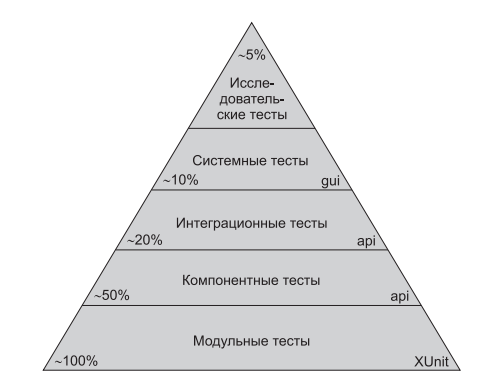
\includegraphics[width=0.9\linewidth]{tests.png}}
\end{frame}
\lecturenotes
Профессиональные разработчики для создания модульных тестов обычно применяют методологию разработки через тестирование (TDD, Test Driven Development). Группы профессиональных разработчиков используют приемочные тесты для составления спецификации своей системы и механизм непрерывной интеграции для предотвращения регрессии. Однако эти тесты составляют лишь часть картины. Какими бы полезными ни были модульные и приемочные тесты, нам также понадобятся тесты более высокого уровня, которые будут следить за тем, чтобы контроль качества не обнаруживал никаких
дефектов. На рис. изображена пирамида автоматизации тестирования — графическое представление всевозможных тестов, необходимых при профессиональной организации разработки.


\section{Управление временем}
\subsection{Сохранение концентрации}
\begin{frame} \frametitle{Сохранение концентрации}
\begin{itemize}
  \item Сон
  \item Кофе
	\item Перерывы
\end{itemize}
\end{frame}
\lecturenotes
Сон\\
Важность сна невозможно переоценить. Профессиональные разработчики управляют своим графиком сна так, чтобы концентрация достигала максимума к тому моменту, когда они утром приходят на работу.\\
Кофеин\\
Несомненно, поглощение умеренных доз кофеина повышает эффективность использования  концентрации. Но будьте осторожны! Кофеин также вводит в вашу концентрацию странную неустойчивость. При избытке кофеина ваше внимание способно смещаться в непредсказуемых направлениях. Слишком сильная кофеиновая стимуляция нередко приводит к тому, что вы тратите весь день, концентрируясь на малозначительных вещах.
Использование и переносимость кофеина — личное дело.\\
Перезарядка\\
Концентрации частично перезаряжается отвлекающими занятиями. Хорошая долгая прогулка, беседа с друзьями, просто взгляд из окна. Одни люди медитируют. Другие выбирают восстановительный сон. Третьи слушают подкасты или листают журналы.

\begin{frame} \frametitle{<<Помидоры>>}
\begin{itemize}
  \item Вы ставите таймер  на 25 минут. Во время работы таймера ничто не должно мешать вашей работе. 
	\item По сигналу таймера-«помидора» вы немедленно прекращаете свою
текущую работу. Пришло время разобраться со всеми проблемами,
возникавшими во время работы таймера.
	\item Каждый четвертый период отдыха делается более продолжительным, 30 минут или около того.
\end{itemize}
\end{frame}
\lecturenotes
Основная идея очень проста: вы ставите стандартный кухонный таймер (традиционно такие таймеры оформляются в виде помидора) на 25 минут. Во время работы таймера ничто не должно мешать вашей работе. Если звонит телефон, вы отвечаете и вежливо просите перезвонить через 25 минут. Если кто-то заходит к вам, чтобы задать вопрос, вы вежливо предлагаете зайти через 25 минут. Независимо от вида прерывания оно откладывается до момента срабатывания таймера. Вряд ли найдется так уж много неотложных дел, которые не могут подождать 25 минут!\\
По сигналу таймера-«помидора» вы немедленно прекращаете свою текущую работу. Пришло время разобраться со всеми проблемами, возникавшими во время работы таймера. Затем вы делаете перерыв примерно на пять минут, снова ставите таймер на 25 минут и начинаете следующий «помидорный» период. Каждый четвертый период отдыха делается более продолжительным, 30 минут или около того.\\
Этот метод управления временем описан достаточно подробно; я рекомендую познакомиться с ним подробнее. Тем не менее даже это краткое описание дает начальное представление об этой методике.\\
При использовании этого метода ваше время делится на продуктивное и непродуктивное. «Помидорное» время продуктивно. Именно в эти периоды выполняется настоящая работа. Остальное время тратится на отвлекающие факторы, встречи, перерывы или другую деятельность, не связанную напрямую с выполнением ваших задач

\subsection{Уклонение от работы}
\begin{frame} \frametitle{Инверсия приоритетов}
\begin{block}{}
Мы убеждаем себя, что у вас есть более срочная задача,
и занимаемся ей. Это называется инверсией приоритетов: вы искусственно повышаете приоритет задачи, чтобы отложить другую задачу,
обладающую настоящим приоритетом.
\end{block}
\end{frame}
\lecturenotes
Независимо от причины мы всегда находим способы избежать выполнения работы. Мы убеждаем себя, что у вас есть более срочная задача, и занимаемся ей. Это называется инверсией приоритетов: вы искусственно повышаете приоритет задачи, чтобы отложить другую задачу, обладающую настоящим приоритетом. Инверсия приоритетов — это ложь, которую мы рассказываем самим себе. Нам не хватает смелости обратиться к тому, что нужно сделать, и мы убеждаем себя, что другая задача более важна. Мы знаем, что это не так, и все же обманываем себя.\\
Хотя правильнее сказать, что мы обманываем не себя. В действительности мы готовим ложь для тех, кто спросит нас, чем мы занимаемся и почему занимаемся именно этим. Мы заранее готовим защиту от мнения других.\\
Конечно, такое поведение непрофессионально. Профессионал оценивает приоритет каждой задачи независимо от своих личных страхов и предпочтений и решает эти задачи в порядке приоритетов.

\begin{frame} \frametitle{Тупики}
\begin{block}{}
Тупик — явление, хорошо знакомое всем разработчикам программных
продуктов. Вы принимаете решение и идете по техническому пути,
который приводит вас в никуда. 
\end{block}
\end{frame}
\lecturenotes
Тупик — явление, хорошо знакомое всем разработчикам программных продуктов. Вы принимаете решение и идете по техническому пути, который приводит вас в никуда. Чем больше упорства вы проявляете в своем решении, чем дальше зайдете на этом пути. А если на кон поставлена ваша профессиональная репутация, то вы будете блуждать вечно.\\
Опыт и благоразумие помогут избежать некоторых тупиков, но обойти их все не удастся. Так что в действительности вы должны быстро понять, что ваш путь завел в тупик, и иметь смелость для отступления. Иногда это называется «правилом ямы»: если вы оказались в яме, прежде всего перестаньте копать.\\
Профессионал не увлекается идеей настолько, чтобы у него не хватило сил отказаться от нее и вернуться к исходной точке. Он непредвзято относится к другим идеям, чтобы у него оставались другие варианты на случай, если он все же окажется в тупике.

\begin{frame} \frametitle{<<Грязь, болота и трясины>>}
\begin{block}{}
Грязь еще хуже, чем тупик. Она вас замедляет, но не останавливает полностью. Грязь препятствует вашему продвижению, но вы все равно можете двигаться вперед, действуя методом «грубой силы». 
\end{block}
\end{frame}
\lecturenotes
Грязь еще хуже, чем тупик. Она вас замедляет, но не останавливает полностью. Грязь препятствует вашему продвижению, но вы все равно можете двигаться вперед, действуя методом «грубой силы». Грязь опаснее тупиков, потому что вы всегда видите путь впереди, и он всегда кажется короче, чем путь назад (хотя на самом деле это не так).\\
Ничто не оказывает более основательного и долгосрочного отрицательного эффекта на
производительность группы программистов, чем грязь в программном коде. Ничто.\\
Проблема в том, что возникновение грязи, как и тупики, неизбежно. Опыт и благоразумие помогут вам избегать его, но рано или поздно вы примете решение, которое заведет вас в грязь. Возникновение грязи весьма коварно. Вы создаете решение простой задачи, всеми силами стремясь к тому, чтобы код оставался простым и чистым. С ростом масштаба и сложности задачи вы расширяете ее кодовую базу, по возможности стараясь сохранять ее чистоту. В какой-то момент вы понимаете, что изначально приняли неверное архитектурное решение и ваш код плохо масштабируется в направлении смещения требований.\\
Здесь и находится критическая точка! Вы все еще можете вернуться и исправить архитектуру. Но вы также можете продолжить движение вперед. Кажется, что возврат обойдется слишком дорого, потому что вам придется перерабатывать существующий код, однако в будущем он обойдется еще дороже. Если вы будете двигаться вперед, то система сползет в грязь, и вполне возможно, что она из нее уже не выберется.\\
Профессионалы опасаются грязи намного сильнее, чем тупиков. Они всегда обращают внимание на грязь, которая начинает неограниченно разрастаться, и прикладывают все необходимые усилия к ее устранению — по возможности раннему и быстрому.\\
Движение вперед по грязи (когда вы знаете, что это грязь) является худшей из разновидностей инверсии приоритетов. Двигаясь вперед, вы обманываете себя, обманываете вашу группу, обманываете свою компанию и заказчиков. Вы говорите им, что все будет хорошо, хотя на самом деле вы ведете их к общей катастрофе.

\begin{thebibliography}{99}
\bibitem{ideal} {Мартин Р. Идеальный программист. Как стать профессионалом разработки ПО./Мартин Р. — СПб.:Питер, 2012. — 224 с.}
\end{thebibliography}

\end{document}

%%% Local Variables: 
%%% mode: TeX-pdf
%%% TeX-master: t
%%% End: 
